%!TEX root = submission.tex

Historical events are difficult to define; historians and political scientists read large quantities of text to construct an accurate picture of a single event.  Events are interesting by definition: they are the hidden causes of anomalous observations.  But they are also inherently abstract---we can observe that changes occur, but we cannot directly observe whether or not an event occurs.

Consider embassies sending diplomatic messages, such as shown in Figure~\ref{fig:cartoon}.  The Bangkok and Hong Kong embassies have \emph{typical concerns} about which they usually send messages.  At date $d$, however, the message content changes for both embassies---again, we only observe the changes in message content, and do not observe the event directly.  Our first goal is to determine \emph{when} events happen, or identify these rare but pervasive deviations from the typical concerns.

Our second goal is to characterize \emph{what} occurs.  We rely on topic models~\cite{Blei:2012} to summarize documents and use that same latent space to characterize events.

We develop a Bayesian model that discovers the typical concerns of authors, identifies when events occur, and characterizes these events; we call this the \emph{Capsule} model, as it encapsulates events.

Our final goal is to visualize the results of the Capsule model to make them accessible.   We provide source code for both Capsule and its associated visualization.

We first review previous research related to event detect, summarization, and visualization.  In Section~\ref{sec:model}, we describe the Capsule model and how to infer the latent parameters (the appendix provides further inference details).  Section~\ref{sec:eval} provides an exploration of results on simulated and three real-world datasets, and we conclude with a discussion in Section~\ref{sec:discussion}.


\begin{figure}
\centering
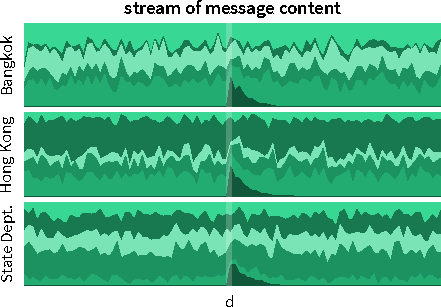
\includegraphics[width=\linewidth]{fig/cartoon.pdf}
\caption{Cartoon intuition of Capsule.  Both the Bangkok and Honk Kong embassies have typical concerns about which they usually send messages (represented in topic space).  When an events occurs at date $d$, the stream of message content alters to include the event, then fades back to ``business as usual.''  Capsule discovers both entities' typical concerns and the event locations and content.}
\label{fig:cartoon}
\end{figure}

% \PP outliers vs events \cite{Neill:2009} (univariate -> multivariate); this whoudlbe in reated work?
% How is event detection different from:
% 1. SupervisedLearning:
% • Abnormal events are extremely rare, normal events are
% plentiful
% 2. Clustering:
% • Clustering = partitioning data into groups
% • Not the same as finding statistically anomalous groups
% 3. OutlierDetection:
% • Events of interest are usually not individual outliers
% • The event typically affects a subgroup of the data rather than a single data point


\parhead{Related work.}  We first review previous work on automatic event detection and other related concepts.  

While Capsule uses text documents and associated metadata as input, event detection is often performed with univariate input data.  In this context, bursts that deviate from typical behavior (e.g., noisy constant or a repeating pattern) can define an event \cite{kleinberg2003bursty,ihler2007learning}; Poisson Processes~\cite{Kingman:1993} are often used to model events under this definition.  Alternatively, events can be construed as ``change points'' to mark when typical observations shift semi-permanently from one value to another~\cite{guralnik1999event}.
In both univariate and multivariate settings, the goal is often the same: analysts want to predict whether or not a rare events will occur~\cite{weiss1998learning,das2008anomaly}.  Capsule, in contrast, is designed to help analysts explore and understand the original data: our goal is interpretability, not prediction.

Text is often used in event detection, as it is an abundant source of data.  
In some applications, documents themselves are considered to be observed events~\cite{mccallum1998comparison,peng2007event}, or events are predetermined and tracked through the documents~\cite{yang2000improving,VanDam:2012}.  We are interested in detecting \emph{unobserved} events which can be characterized by patterns in the data.

A common goal is to identify clusters of documents; these approaches are used on news articles~\cite{zhao2012novel,zhao2007temporal,zhang2002novelty,li2005probabilistic,wang2007mining,allan1998line} and social media posts~\cite{VanDam:2012,lau2012line,jackoway2011identification,sakaki2010earthquake,reuter2012event,becker2010learning,sayyadi2009event}.  
In the case of news articles, the task is to create new clusters as novel news stories appear---this does not help disentangle typical content from rare events of interest.
Social media approaches identify rare events, but the methods are designed for short, noisy documents; they are not appropriate for larger documents that contain information about a variety of subjects.

Many existing methods use document terms as features, frequently weighted by tf-idf value~\cite{fung2005parameter,kumaran2004text,brants2003system,das2011dynamic,zhao2007temporal,zhao2012novel}; here, events are bursts in groups of terms.  Because language is high dimensional, using terms as features limits scalability.

Topic models~\cite{Blei:2012} reduce the dimensionality of text data; they have been used to help detect events mentioned in social media posts~\cite{lau2012line,dou2012leadline} and posts relevant to monitored events~\cite{VanDam:2012}.
We rely on topic models to characterize both typical content and events, but grouped observations can also be summarized directly~\cite{peng2007event,chakrabarti2011event,gao2012joint}.

In addition to text data over time, author~\cite{zhao2007temporal}, news outlet~\cite{wang2007mining}, and spatial information~\cite{Neill:2005,mathioudakis2010identifying,liu2011using} can be used to augment event detection.  Capsule uses author information in order to characterize typical concerns of authors.

Detecting and characterizing relationships~\cite{schein2015bayesian,linderman2014discovering,das2011dynamic} is related to event detection.  When a message recipient is known, Capsule's author input can be replaced with a sender-receiver pair, but the model could be further tailored for interactions within networks.

Once events have been identified and characterized, visualization translates a model's output into sometime intepretable for non experts.  LeadLine~\cite{dou2012leadline} is an excellent example of a visualization of event detection.  We build on topic model visualization concepts~\cite{chaney2012visualizing} to provide tailored visualization code for Capsule.